
\section{Motivation}
\begin{frame}{ motivation}
%\textsf{例} \textbf{例}  \textit{例}
% \texttt{例}  % 调出仿宋字体了
%\begin{table}[]
%\caption{PMT performance qualification standard}
%\resizebox{.8\textwidth}{!}{%
%\begin{tabular*}{.98\textwidth}{l|c|c}
%%\toprule
%\hline
%\hline
%parameter & HAMAMATSU PMT&NNVT PMT\\
%\hline
%HV@Gain=$10^7$ &  <2350 V&<2800V \\
% PDE & >24\%& >24\%\\
% DCR & <50kHz& <100kHz\\
% PV & >2.5& >2.5\\
% rise time & <8.5ns& --\\
% fall time & <12ns&-- \\
% FWHM & ----& --\\
% resolution & <0.4&<0.4 \\
%\hline
%\end{tabular*}
%}
%\end{table}
\begin{enumerate}
\item 	The Raw data of PMT testing is significant for the evaluation of PMT performance. 
\item \textbf{While,Currently, the raw data of container system is not well organized and it is  not convinent for people to get a quikly access.  }
\item \alert{It is useful to convert all the testing raw data to ROOT format.}
\begin{itemize}
\item decrease the file size
\item easy to analysis and manage.
\item shadow the hardware details.
\end{itemize}
\end{enumerate}
%\begin{figure}
%\centering
%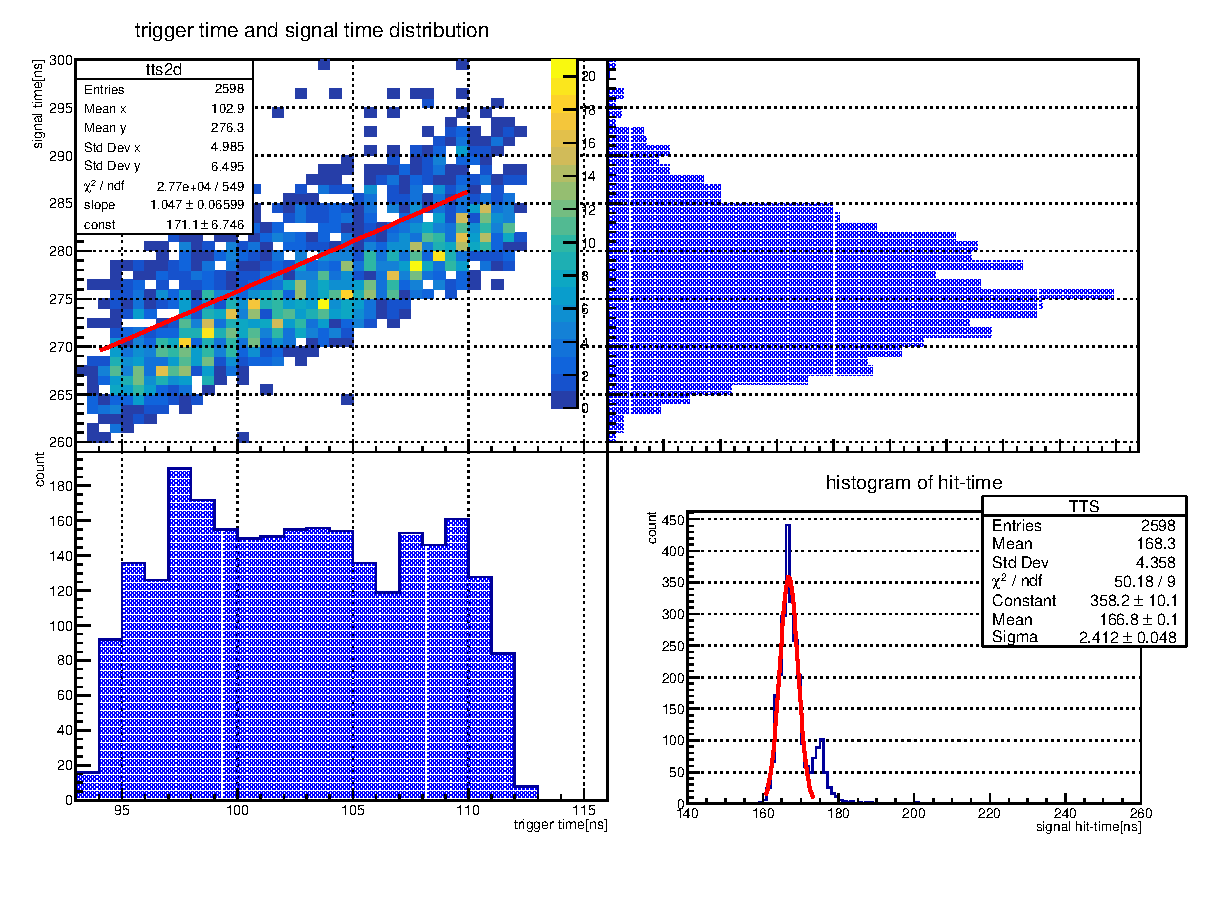
\includegraphics[width=0.78\textwidth]{typical_hittime} % 单图
%\end{figure}
\end{frame}
%%%%%%%%%%%%%%%%%%%%%%%%%%%%%%%%%%%%%%%%%%%
\begin{frame}{requirements}
\begin{enumerate}
\item sotre the raw waveform data(.1pe, 1pe, TTS).
\item store the auxilary testing information(container #, mass#, HV, DCR. etc).
\item easy to manage (create, modify and update) and analyze.
\item \alert{one ane acquire almost all the data needed for analysis(of one PMT) from only one file} rather than collecting the details from server.

\end{enumerate}
beloew is the figure about 
\end{frame}
%%%%%%%%%%%%%%%%%%%%%%%%%%%%%%%%%%%%%%%%%%%
\begin{frame}{prliminary file structure and stretages}
\begin{itemize}
\item each PMT have one root file named in "SN\_rawdata.root"
\item In a specific root file, we have several trees and a auxilary data class
\item if one PMT go through several tests in the container, all the data will be saved still in only one root file but with different name of trees\footnote{distiguished by a unique tag}. 
\end{itemize}

\end{frame}
%%%%%%%%%%%%%%%%%%%%%%%%%%%%%%%%%%%%%%%%%%%
\begin{frame}{results}
current file path:
the folder MCP contains all the MCP PMT data files;
the folder HAMAMATSU contains all the  HAMAMATSU data files;
 
\end{frame}
%%%%%%%%%%%%%%%%%%%%%%%%%%%%%%%%%%%%%%%%%%%
%\begin{frame}{calibration of each drawer}
%Generally, we put several PMTs with known PDE value\footnote{or QE value}  into one drawer and linearly fit the PDE-$\mu_{test}$ data to get \alert{drawer$_{factor}$}.
%\vspace{.5cm}
%\hrule{\textwidth}
%\vspace{.5cm}
%
%While an alternative way to access the drawer$_{factor}$ is fitting PDE-$\mu_{test}$ data {\color{red}from all the PMTs tested in one drawer rather than the mannual selected ones.} Then once we finish one PMT test in a drawer we will get one more statistical sample in the PDE-$\mu_{test}$ fitting, and we could expect that the fitted drawer$_{factor}$ will get more stable as we testing more PMTs.
%
%\vspace{.5cm}
%The advantage of this "self-calibration" method is that we could {\color{red}decrease the statistical error as much as possible}; and the remained fluctuation of drawer$_{factor}$ can be the system error.
%\end{frame}
%\section{Waveform and Charge Spectrum}
%%%%%%%%%%%%%%%%%%%%%%%%%%%%%%%%%%%%%%%%%%%
%\begin{frame}{抽屉刻度方法}
%滨松厂家提供部分PMT的QE\footnote{假定所有的PMT的收集效率相同}值,可以从PMT数据库\footnote{王俊[http://pmtdb.juno.ihep.ac.cn/index.html]}查询到。如果某一个抽屉测到的滨松PMT恰好有QE的厂家值,就选用它进行刻度。
%
%\vspace{.5cm}
%\hrule{\textwidth}
%\vspace{.5cm}
%为了保证刻度PMT的性能,只选取通过集装箱测试的PMT进行刻度。
%\end{frame}
%%%%%%%%%%%%%%%%%%%%%%%%%%%%%%%%%%%%%%%%%%%
%\begin{frame}{一个抽屉的刻度结果}
%随着测试PMT数量的增加,拟合统计误差逐渐减小,$drawer_{factor}$的拟合结果趋于稳定(更多抽屉拟合结果见back-up部分)。
%\begin{figure}
%\centering
%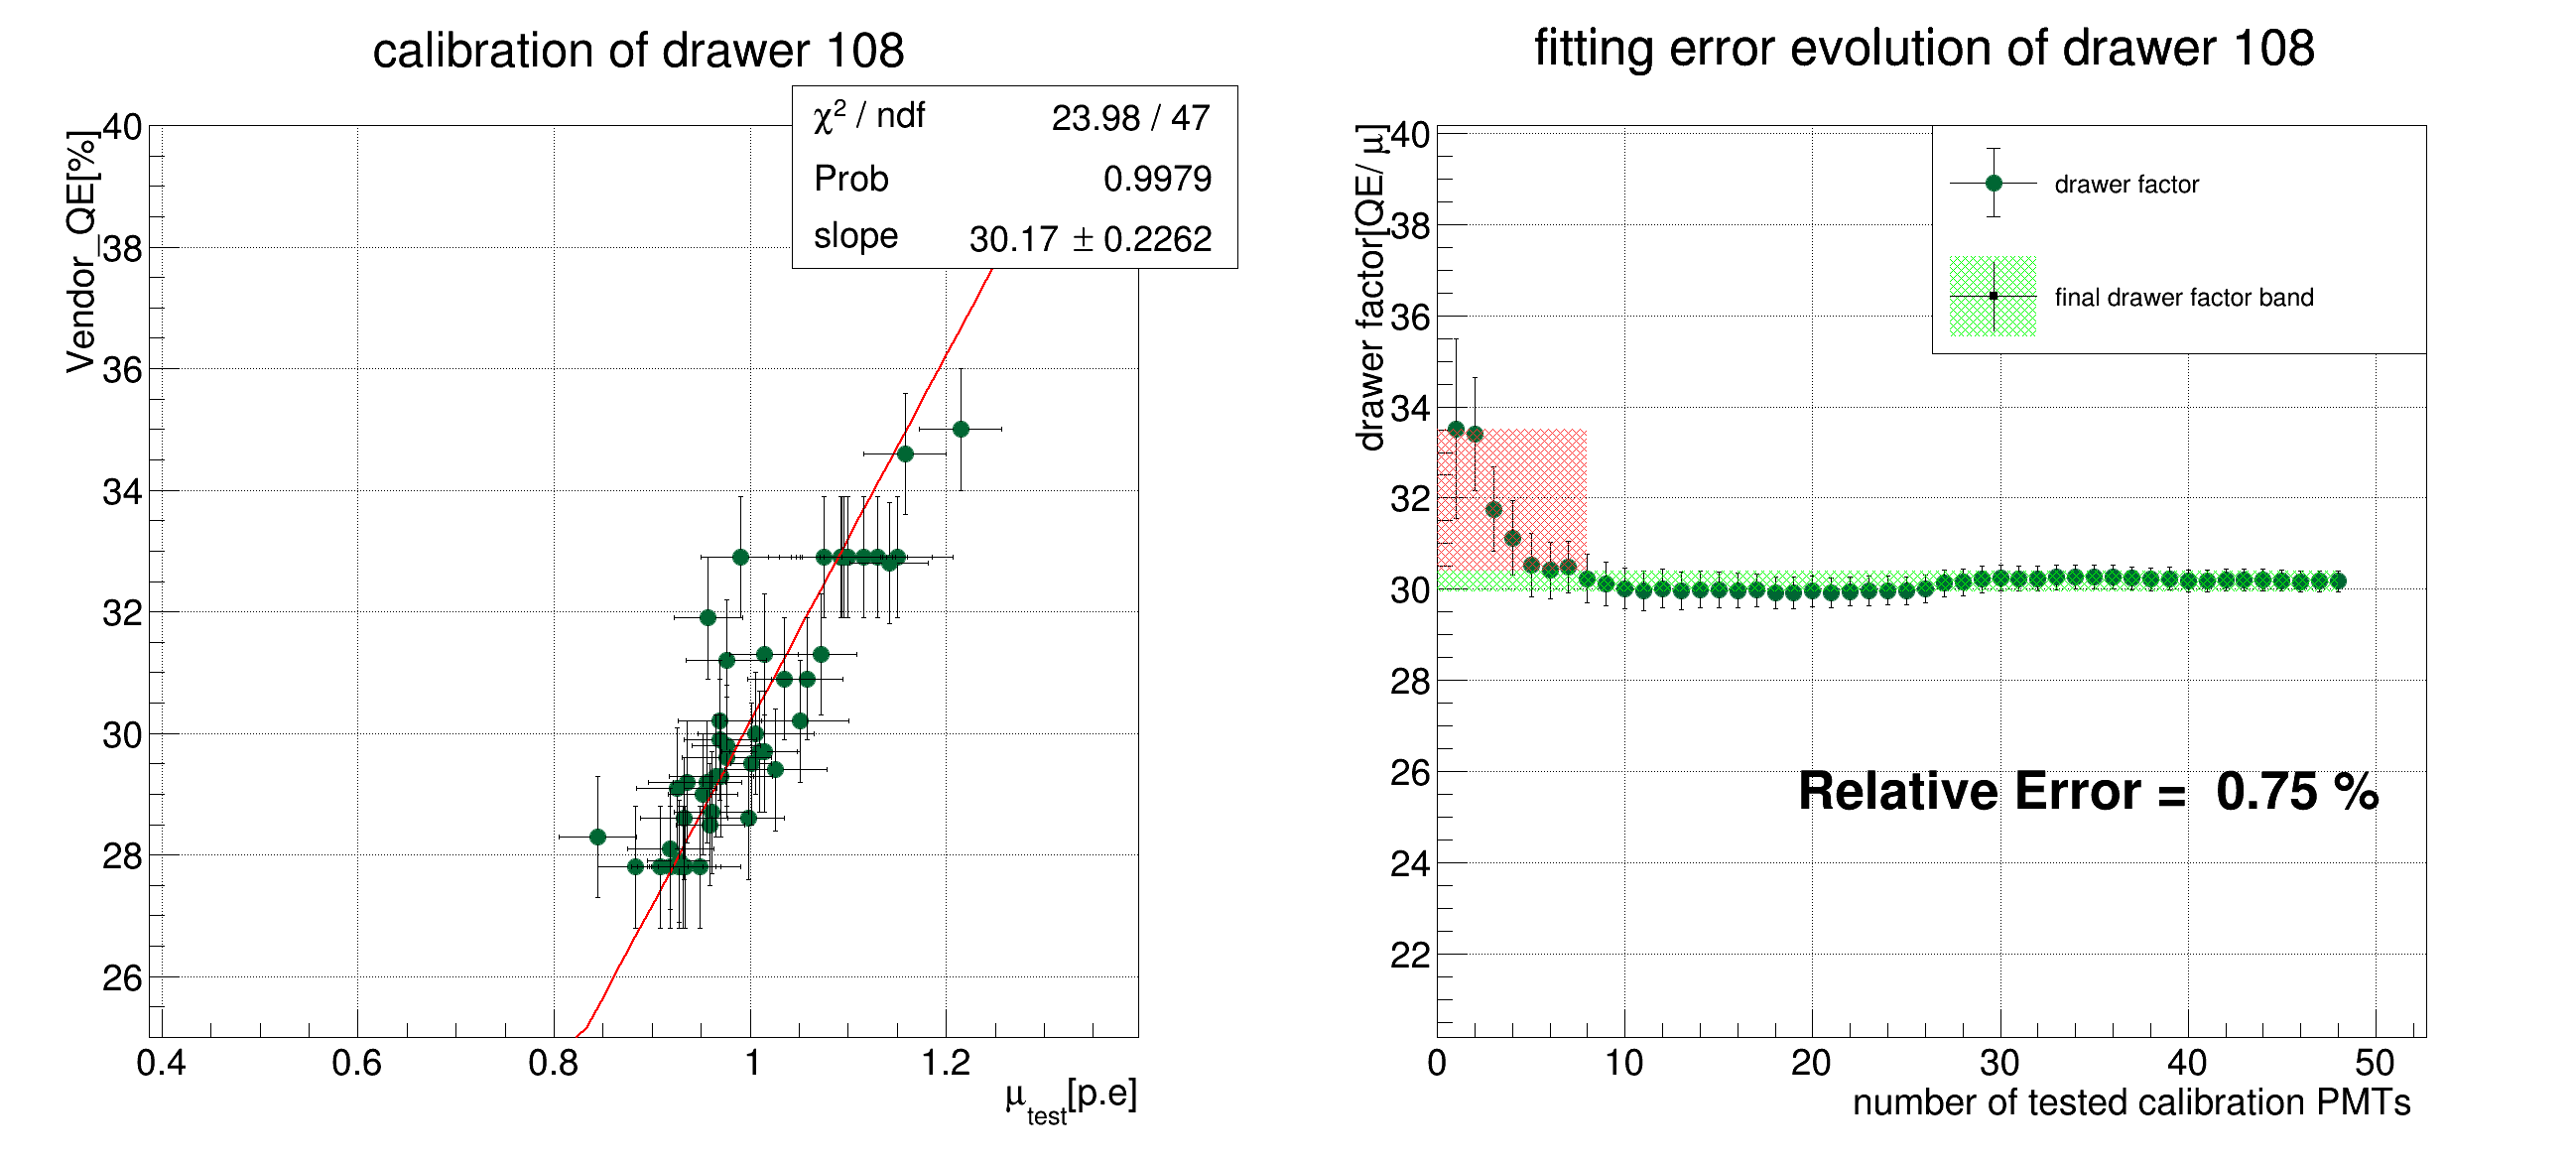
\includegraphics[width=0.98\textwidth]{sta101-7} % 单图
%\caption{108抽屉的$drawer_{factor}$拟合结果}
%\end{figure}
%\end{frame}
%%%%%%%%%%%%%%%%%%%%%%%%%%%%%%%%%%%%%%%%%%%
\begin{frame}{example C++ code of reading the file}
listing
figure
\end{frame}
%%%%%%%%%%%%%%%%%%%%%%%%%%%%%%%%%%%%%%%%%%%
%%%%%%%%%%%%%%%%%%%%%%%%%%%%%%%%%%%%%%%%%%%%%%%%%%%%%%
\section{Summary}

\begin{frame}{summary}
\begin{itemize}
\item  the charge and amplitude stability of HAMAMATSU PMT is better.
\item  $\sim$6k NNVT PMTs and 5k HAMAMATSU PMTs has been tested in container system, test results and test reports are avaliable from PMTDataBase\footnote{pmtdb.juno.ihep.ac.cn}.
\item we reject or accept one PMT according to its perfomance test results from container and scanning station.
\item  {\color{red}we need to study the "delay signal" of HAMAMATSU PMT and "big signal" of NNVT PMT\footnote{especially when PMT working in the multi-photon case}} in detail\footnote{one option is to transport several PMTs to SYSU for detailed study}.
\item the expected mean PDE value is 30.4\% and mean DCR value is $\sim$34kHz\footnote{will decrease after installation} in CD.
%\item 保存重要的测试信息和输出结果到PMT数据库,所有测试结果\footnote{包含集装测试历史数据}可以直接通过http://pmtdb.juno.ihep.ac.cn/\footnote{Query::LPMT Tested Reports} 查询得到
%\item 初步结论:目前现场5002支滨松PMT,382支外观检测不合格,5支HV不合格,2支波形较差,24支DCR不合格,9支PDE不合格。
\end{itemize}
\end{frame}

\begin{frame}
\centering {\zihao{0} \color{red} {THANKS}}
\end{frame}

\begin{frame}
\centering {\zihao{0} \color{red} {BACK-UP}}
\end{frame}

%\begin{table}[htbp]
%\caption{PMT typical performance}
%\resizebox{.8\textwidth}{!}{%
%\begin{tabular*}{.98\textwidth}{l|cccc}
%%\toprule
%\hline
%\hline
%Performance & PDE &DCR & TTS& uniformity \\
%\hline
%HAMAMATSU &  lower\% & 20 kHz& 3ns& worse \\
%NNVT  & higher\% & 40kHz & 7ns& better \\
%\hline
%\end{tabular*}
%%}
%\end{table}

%\end{frame}
%%%%%%%%%%%%%%%%%%%%%%%%%%%%%%%%%%%%%%%%%%%%%%%%%%%%%%
\begin{frame}{TTS of HAMAMATSU PMT}
\begin{figure}
\centering
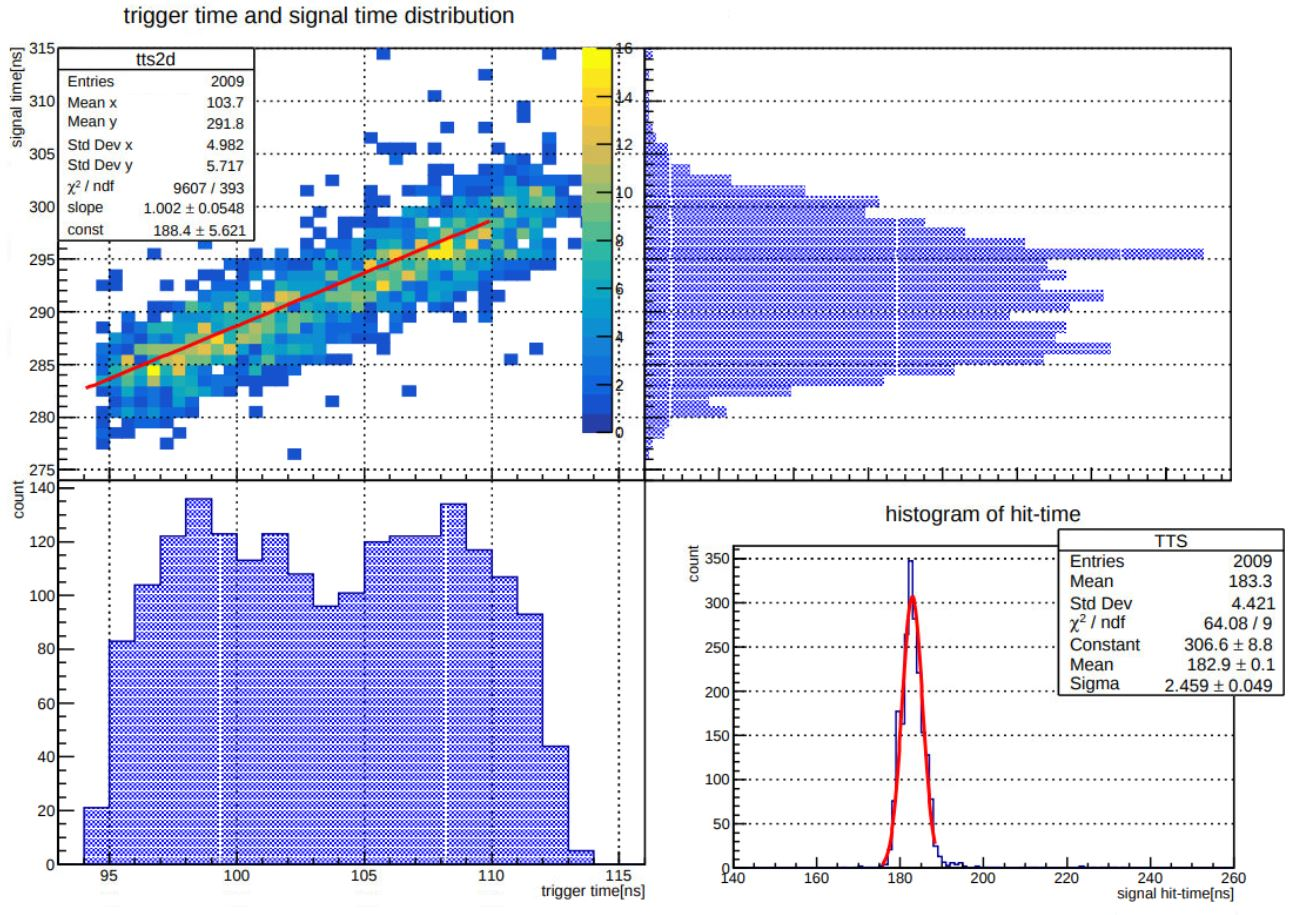
\includegraphics[width=.8\textwidth]{figures/hamtts.JPG} % 单图
%\label{fig:wave2d}
\caption{hittime and trigger time}
\end{figure}
\end{frame}
%%%%%%%%%%%%%%%%%%%%%%%%%%%%%%%%%%%%%%%%%%%%
%%%%%%%%%%%%%%%%%%%%%%%%%%%%%%%%%%%%%%%%%%%%%%%%%%%%%%%%%%%%%%%%%%%%

\appendix

\section*{附录}
